\section{Visualizing the dynamics of vortices in a 2D Bose gas}

The given routine creates vortices, differing in charge $n$, also known as winding number and arrangement. We try out some constellations including only single quantized vortices, vortex-antivortex pairs and vortices with higher charges. The evolution of the resulting densities and the corresponding phase distributions is depicted in the following. 

\subsection{Vortex-Antivortex pairs with the same charge}
 \begin{figure}[H]
 \centering
 \begin{subfigure}{0.49\textwidth} 
 	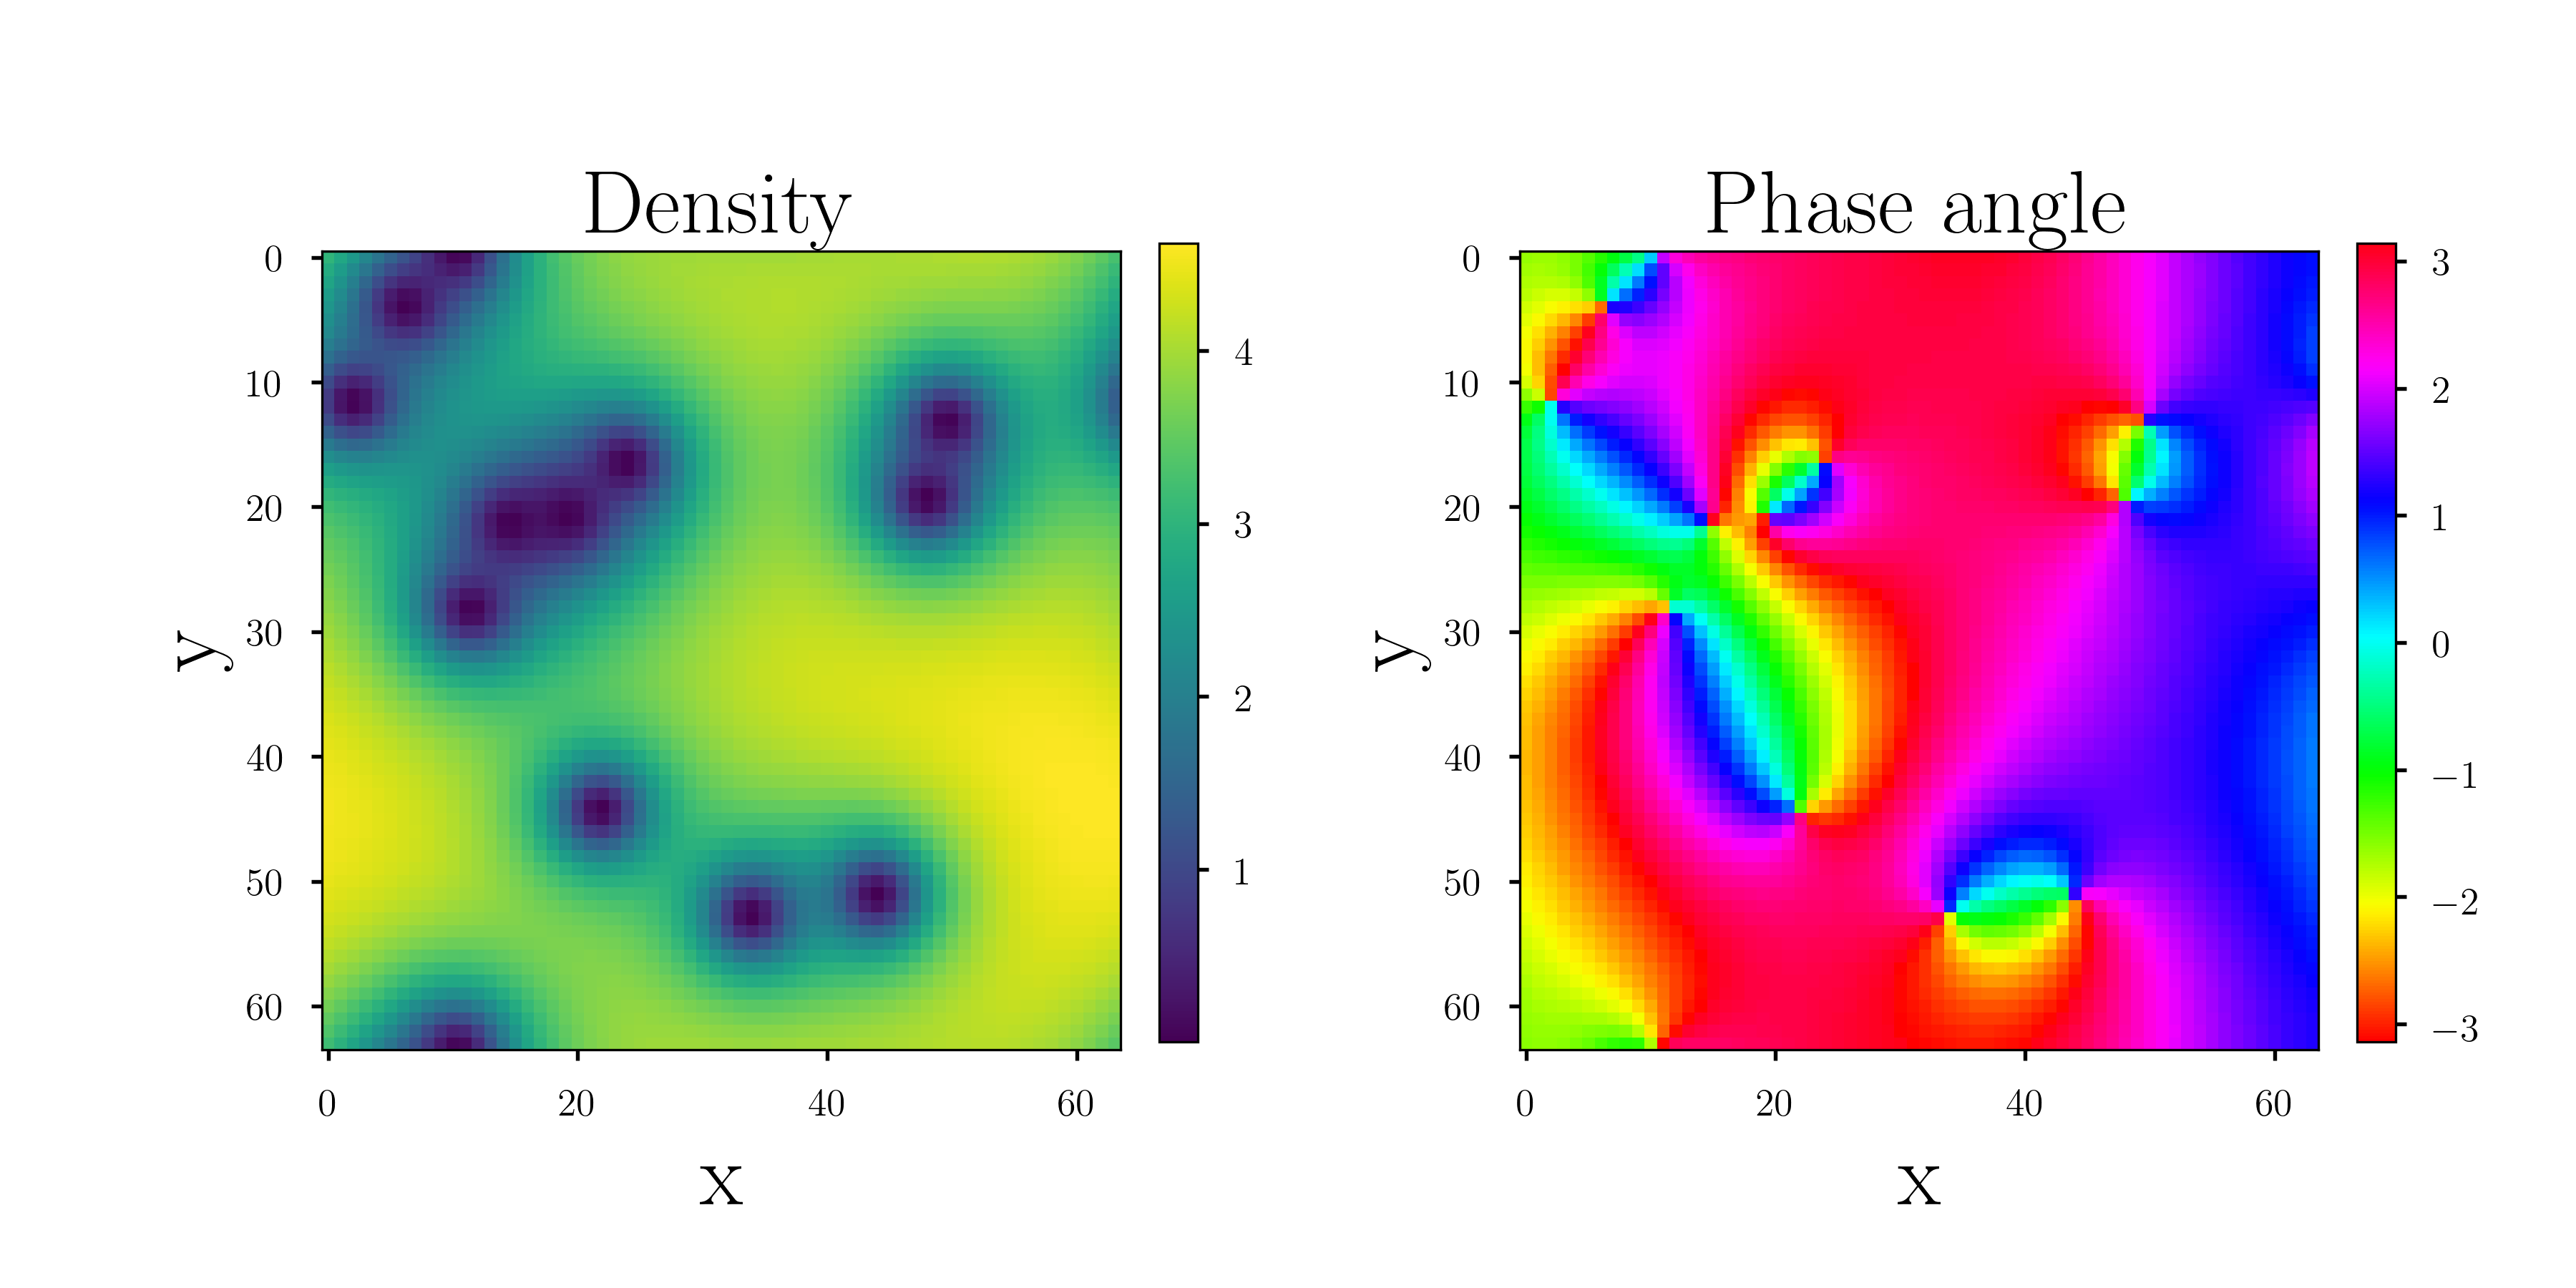
\includegraphics[width= \textwidth]{figures/vortex_1_0}
 	\subcaption{Initial state}
 \end{subfigure} 
 \begin{subfigure}{0.49\textwidth} 
 	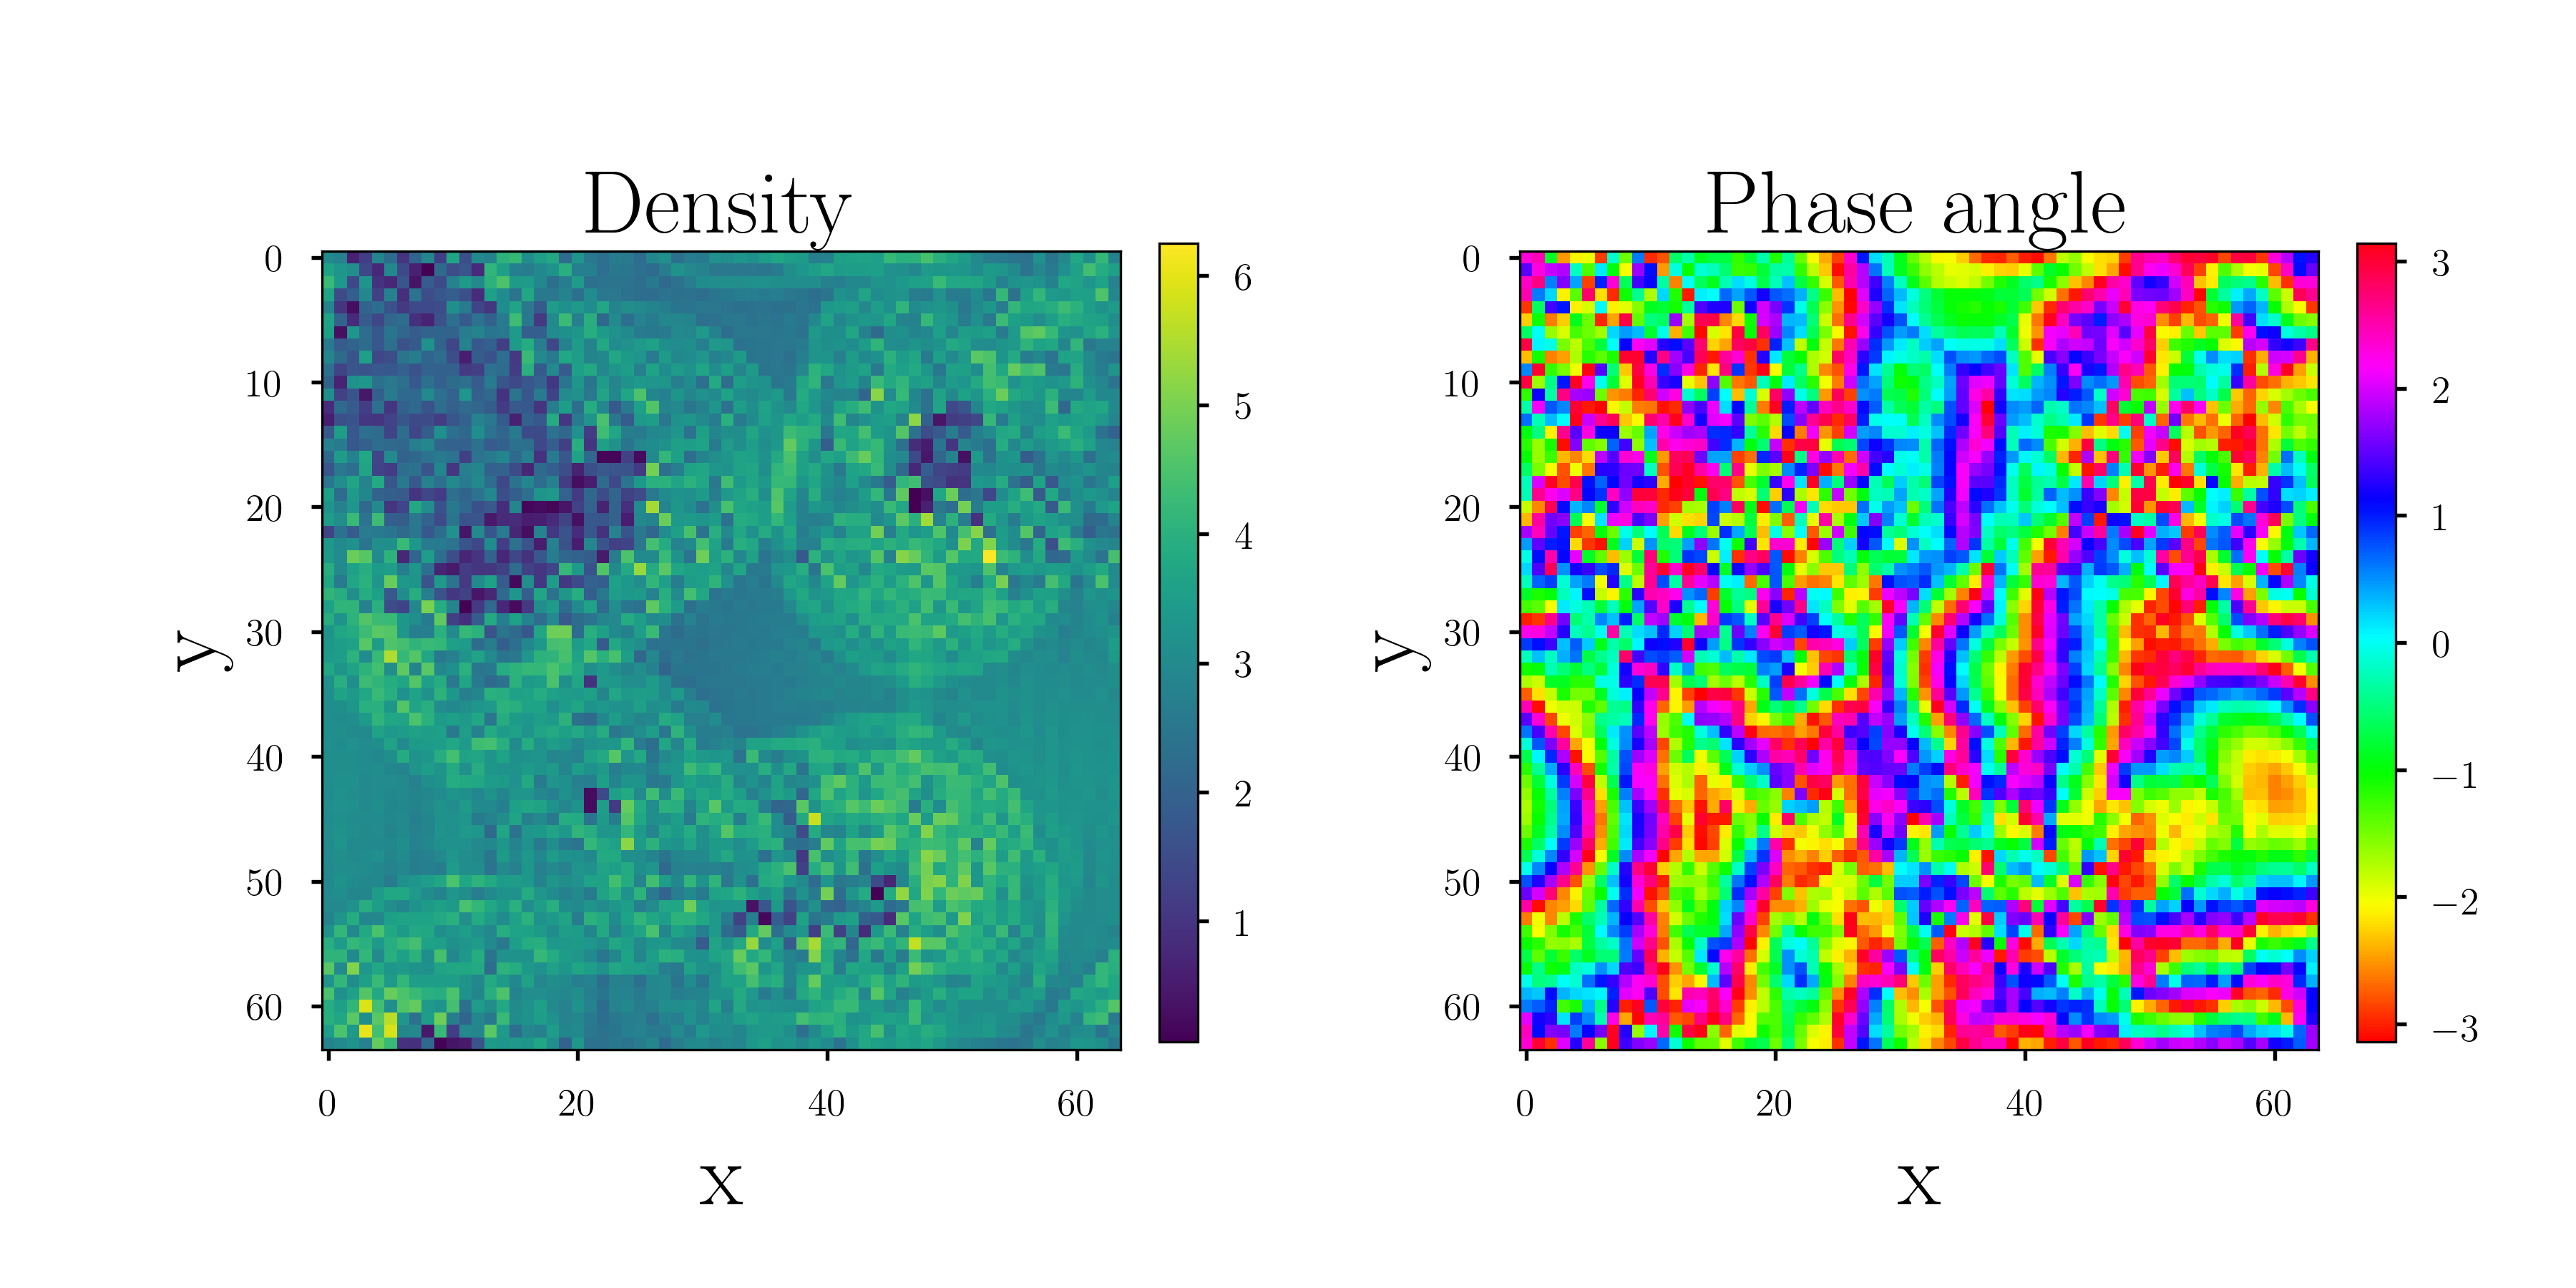
\includegraphics[width=\textwidth]{figures/vortex_1_50}
 	\subcaption{After $N_{\text{steps}} = 50$.}
 \end{subfigure}
 \caption{Dynamics of vortex-antivortex pairs.}	
 \end{figure}

\subsection{Randomly placed vortices with higher charges}
 \begin{figure}[H]
 \centering
 \begin{subfigure}{0.49\textwidth} 
 	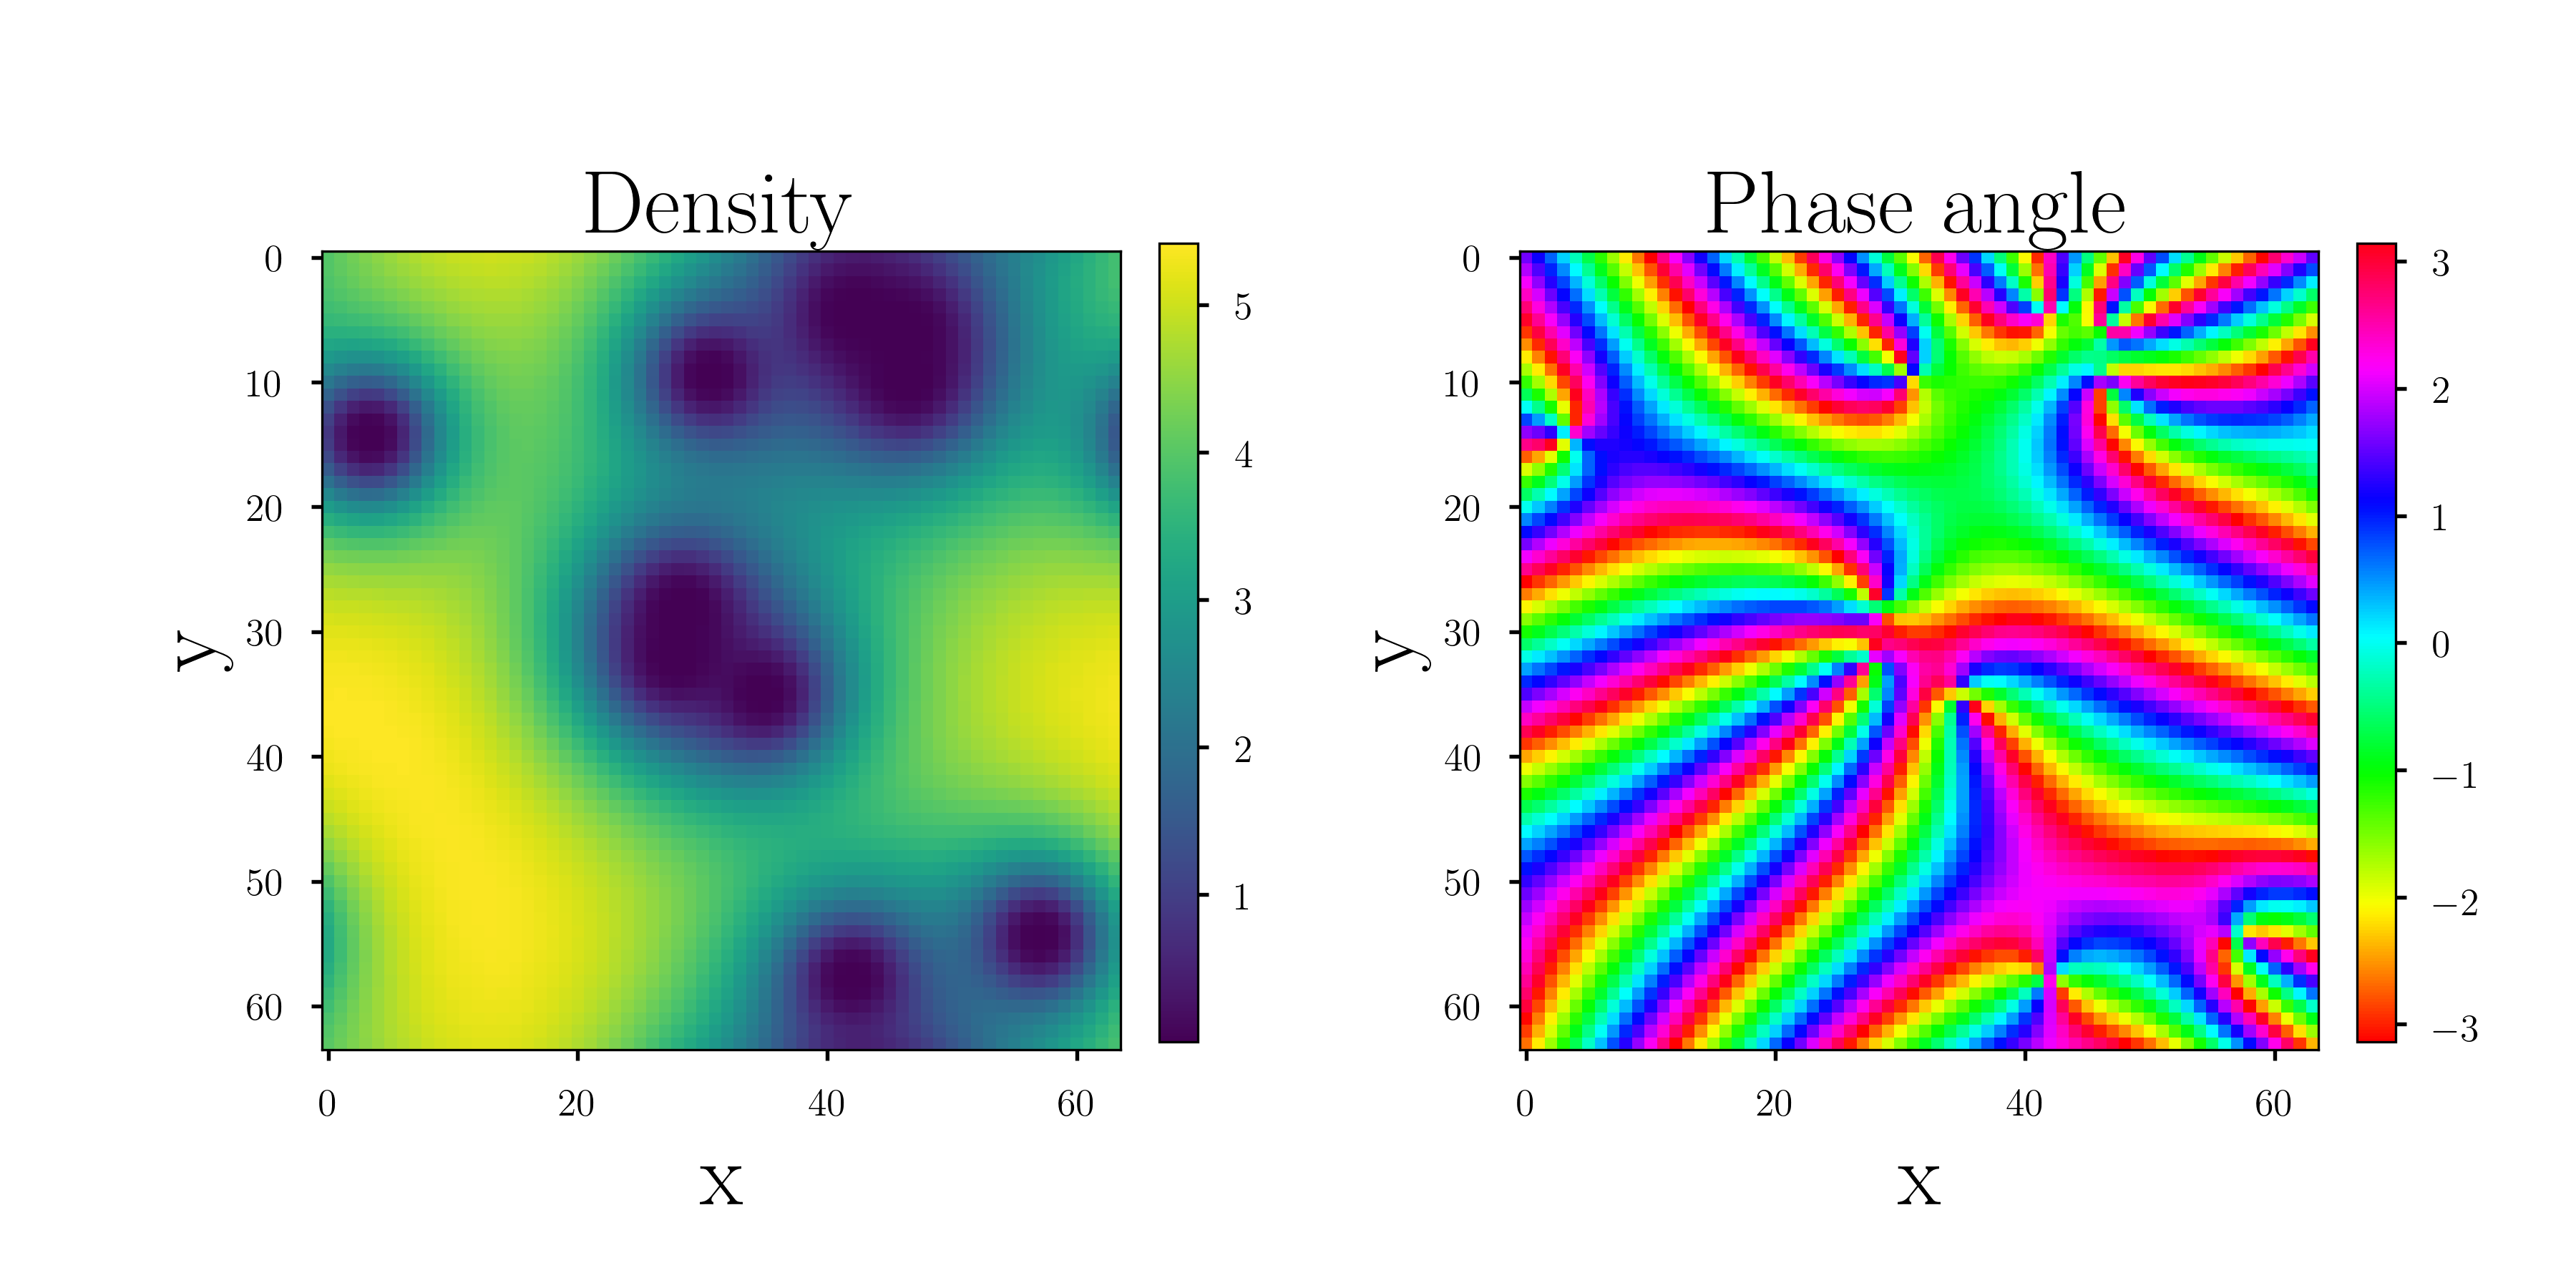
\includegraphics[width= \textwidth]{figures/vortex_2_0}
 	\subcaption{Initial state}
 \end{subfigure}
 \begin{subfigure}{0.49\textwidth} 
 	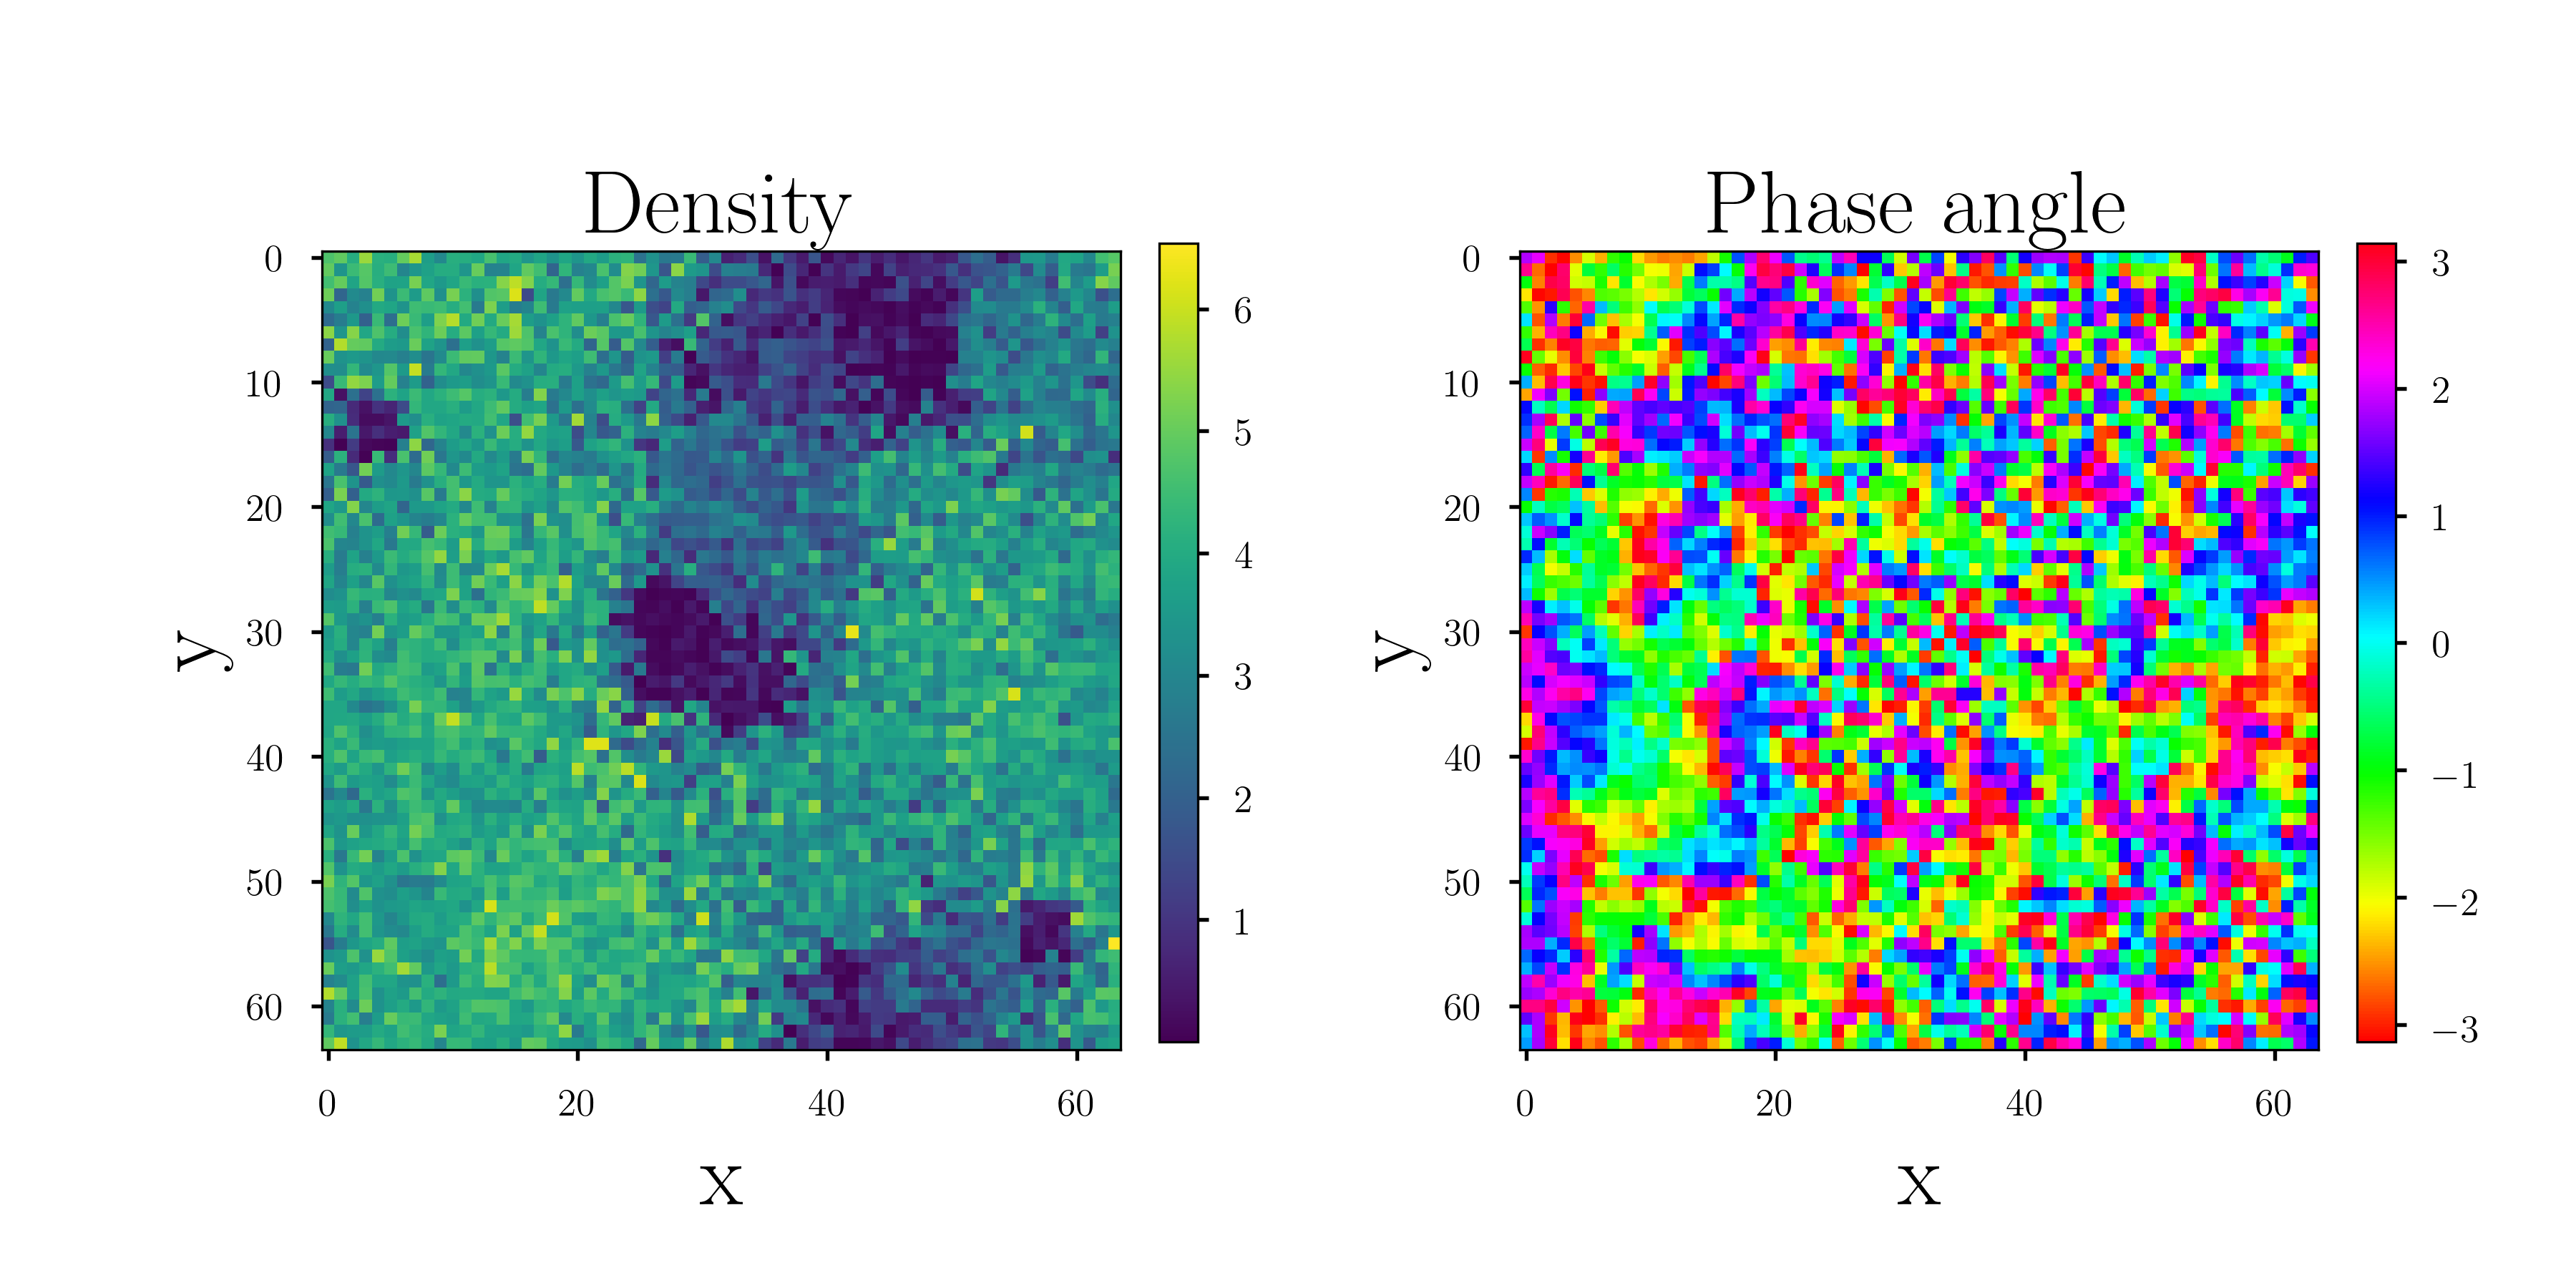
\includegraphics[width= \textwidth]{figures/vortex_2_80}
 	\subcaption[(b)]{After $N_{\text{steps}} = 80$.}
 \end{subfigure}
 \caption{Dynamics of vortices with higher charges.}	
 \end{figure}
 
\subsection{Equidistant placement of vortices with higher charges}
 \begin{figure}[H]
 \centering
 \begin{subfigure}{0.49\textwidth} 
 	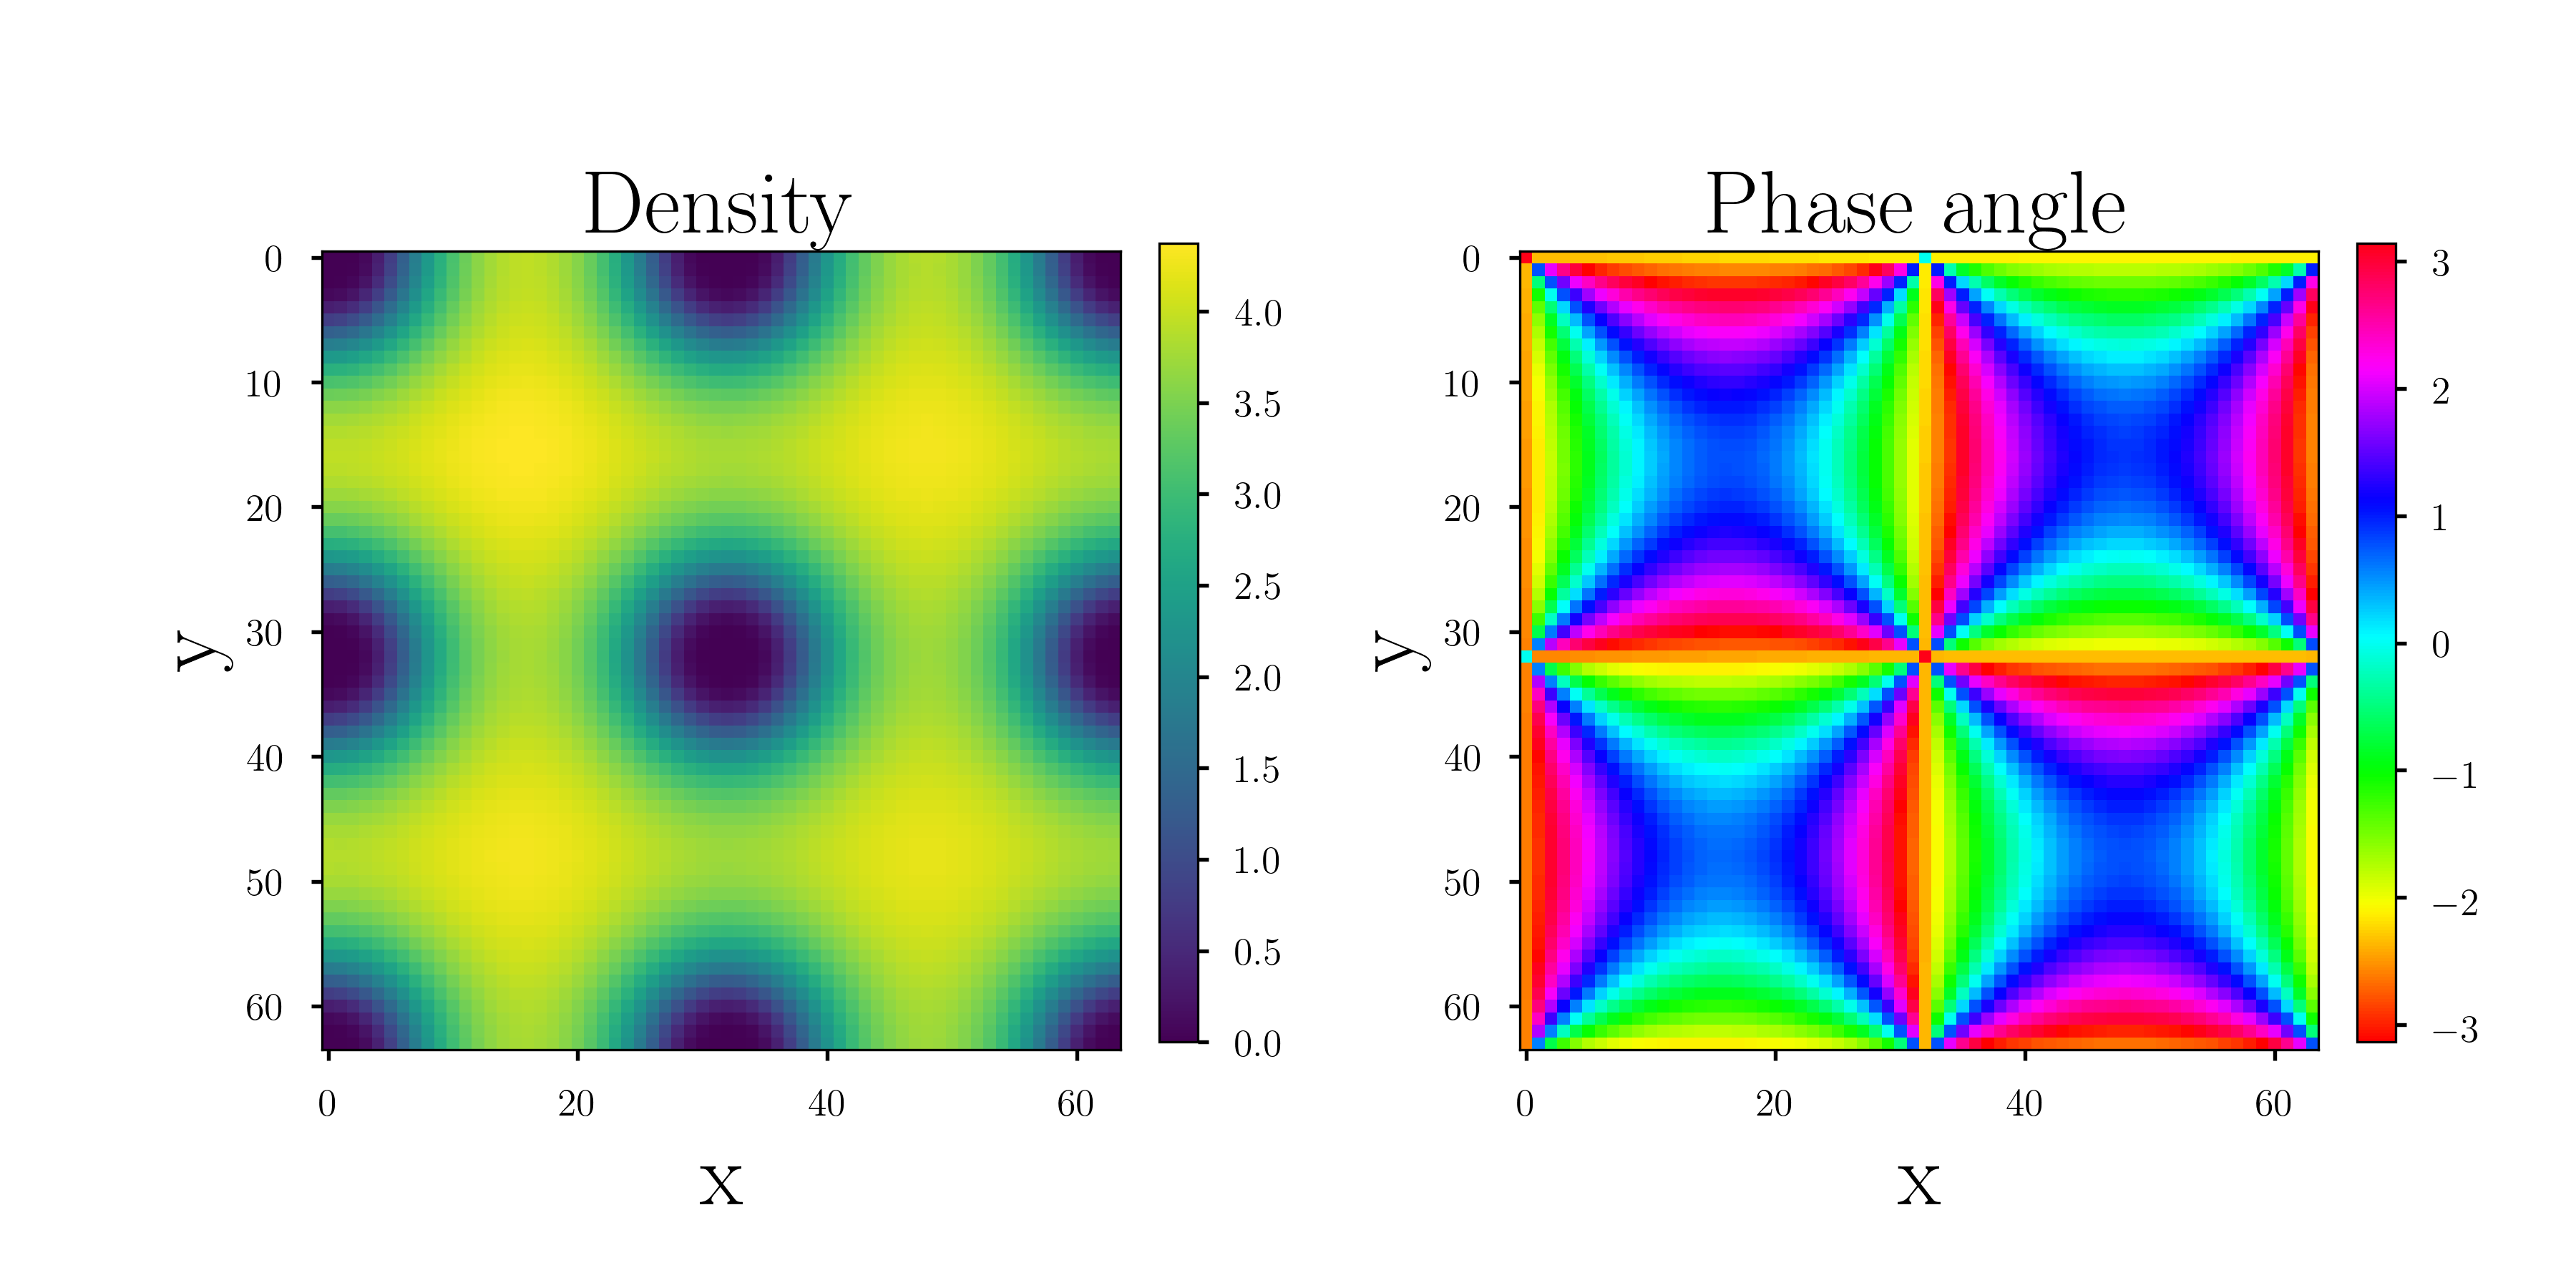
\includegraphics[width= \textwidth]{figures/vortex_3_0}
 	\subcaption{Initial state}
 \end{subfigure}
 \begin{subfigure}{0.49\textwidth} 
 	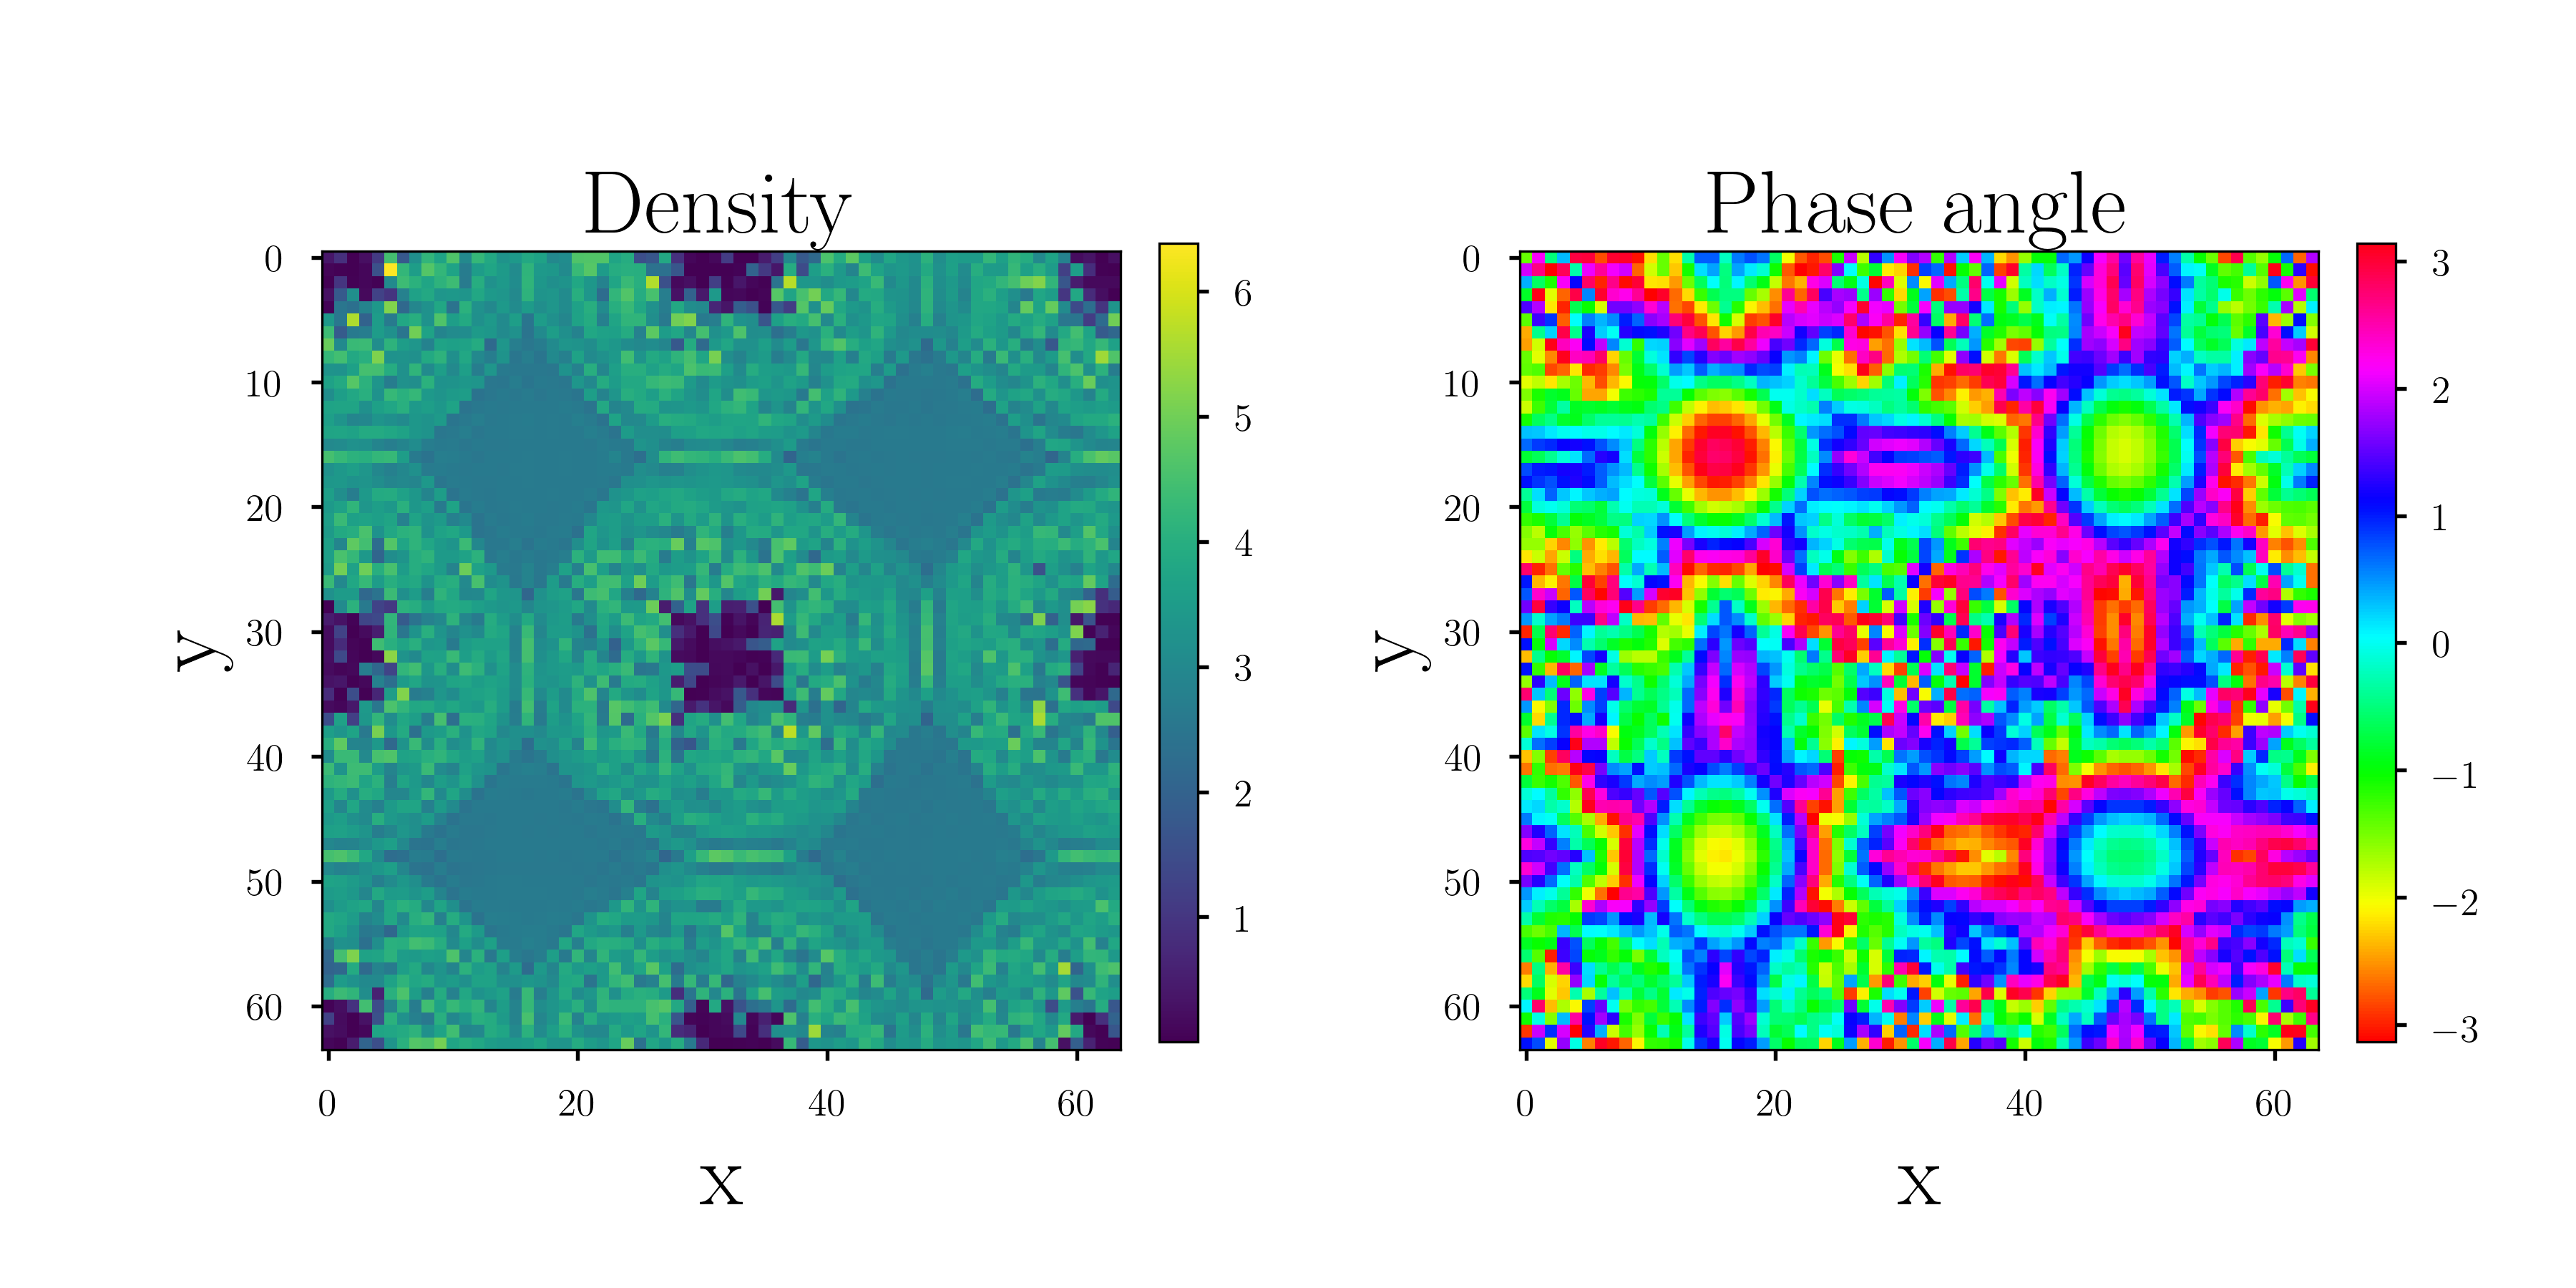
\includegraphics[width= \textwidth]{figures/vortex_3_50}
 	\subcaption{After $N_{\text{steps}} = 50$.}
 \end{subfigure}
 \caption{Dynamics of an ordered initial state of solitons with higher charges.}	
 \end{figure}